\documentclass[10pt,twocolumn,letterpaper]{article}

\usepackage{cvpr}
\usepackage{times}
\usepackage{epsfig}
\usepackage{graphicx}
\usepackage{amsmath}
\usepackage{amssymb}

% Include other packages here, before hyperref.

% If you comment hyperref and then uncomment it, you should delete
% egpaper.aux before re-running latex.  (Or just hit 'q' on the first latex
% run, let it finish, and you should be clear).
\usepackage[breaklinks=true,bookmarks=false]{hyperref}

\cvprfinalcopy % *** Uncomment this line for the final submission

\def\cvprPaperID{****} % *** Enter the CVPR Paper ID here
\def\httilde{\mbox{\tt\raisebox{-.5ex}{\symbol{126}}}}

% Pages are numbered in submission mode, and unnumbered in camera-ready
%\ifcvprfinal\pagestyle{empty}\fi
\setcounter{page}{1}
\begin{document}

%%%%%%%%% TITLE
\title{Deep Network Defined Error Correcting Code}

\author{Gan Tu\\
UC Berkeley\\
{\tt\small tugan@berkeley.edu}
}

\maketitle
%\thispagestyle{empty}

%%%%%%%%% ABSTRACT
\begin{abstract}
   Modern error correcting codes are used in wireless radio communications in order to detect and recover corrupted bits sent over noisy channels. Viterbi algorithm has been the popular decoding algorithm used for such purposes for its optimality. However, many of the algorithms used for radio nowadays depend on predefined scheme such as Trellis and generator matrices. In this research, I explored the possibility of a deep neural network based approach to error correction, as an initial effort towards the goal of an end-to-end radio communication scheme in future. Specifically, I will briefly recap what I did this semester, what I learned, and what I found interesting in this report. I will also demonstrate some initial results obtained for convolutional encoding error correction by Feed Forward Neural Networks, Convolutional Neural Networks, Long Short Term Memory Networks (LSTM), and Bidirectional-LSTMs, compared against baseline optimal Viterbi decoding algorithm. I will also propose a new unexplored ResNet-based architecture for future research efforts.
\end{abstract}


%-------------------------------------------------------------------------
\section{Experiments}

As an initial effort to examine the plausibility of a deep network based approach to error correcting codes, I trained and evaluated multiple common basic neural network architectures on this task. In this section, I will introduce the data source generated and used for training, explain the architecture design and relevant choices made, demonstrate the performance of each architecture, and compare them against each other and the optimal Viterbi decoding baseline.

\subsection{Data Source}
I generated 25,000 data points for the architecture exploration, training, and development. Each data point consists of a random message of k bits, its convolutional encoding, the corrupted encoding after a noisy binary symmetric channel, and it's corresponding Viterbi decoding results. To generate a random message of k bits, a sequence of k bits is randomly drawn from a Bernoulli distribution with a mean $p=0.5$ probability for being the 1 bit. Then, the sequence is convolutionally encoded with a Trellis of 3 and a rate of 1/2, generated using a common generator matrix of $\begin{bmatrix}5 \\ 7\end{bmatrix}$ (credits to pg. 789-790, Proakis and Salehi 2nd edition). Then, this encoded sequence is passed to a binary symmetric channel with varying corruption probabilities. In this report, I will showcase the results for both a low corruption channel ($p=0.05$) and a high corruption channel ($p=0.15$). Finally, the corresponding Viterbi sequences are also recorded.

\subsection{Training}
The experiments and models are implemented in Keras with Tensorflow backend. During training, a train-validation-test split of 0.2-0.2-0.6 is used. In other words, models are trained on 15,000 data points, validated on 5000 data points, and tested on 5000 data points for each result shown later. All the data are shuffled before performing the data splits. For each experiment, all architecture and models are trained on the \textbf{same} set of train-validation-test data sets in order to demonstrate unbiased result of different model performance without the fluctuations in model performance due to different data shuffling.

\subsection{Loss Function}

I treat the problem of decoding as a binary classification problem of classifying whether each output bit is 0 or 1, so I used binary cross entropy as the loss function in which we optimize on. Other loss functions such as mean squared error are also examined, but perform poorly compared to the proposed binary cross entropy loss.


\subsection{Feed Forward Neural Networks}

Because Feed Forward Neural Networks (FNN) is less computational heavy compared to other neural network architectures, I conducted a simple grid search on the size of hidden layers and the number of layers to use. Specifically, I searched over the FNN architecture space from 1 hidden layer to 4 hidden layers (excluding output layer) with varying hidden layer size (from 32 to 1024 nodes at 2x increment). From observation, most three-layer FNNs work similarly well but architectures with 32 to 128 hidden nodes size work slightly better. Upon comparison and empirical performance, a 32-64-128-output architecture choice is used for data of message length $k=10$ and low channel corruption probability of $p=0.05$. For larger message length data, the hidden layers are correspondingly linearly increased, with proper adjustment to regularizations. Specifically, for longer message length $k=40$, a 128-256-480-output architecture is used.

\subsection{Convolutional Neural Networks}

Convolutional Neural Networks (CNN) seem very intuitive in this problem because the encoded message itself is convolutionally encoded and the use of CNN for decoding should work well. Empirical experiments exactly confirmed this assumption. However, when designing the neural network architecture, one caveat is required to be considered due to the nature of input data. CNNs are usually used for image related tasks, which come in as 3 dimensional image input. However, an encoded sequence is just an array of bits so they come in as 1 dimensional vectors. Therefore, I choose to use 1D convolution instead of 2D convolutions for this task, as it also intuitively makes sense as it's a classic signal processing task, but 1D convolution alone is not enough. 

1D convolution in Keras still expect 2D dimensional inputs, so I made a seemingly unintuitive decision by reshaping all the $1 \cdot K$ 1D sequence vector to $6 \cdot \frac{K}{6}$ 2D matrices. The reason behind this reshape is that inputs are encoded using a Trellis of 3, so a row length of 6 helps capture enough information both before and after each Trellis 3 window. Empirically it indeed works well. Note, I also tried using other window sizes and reshape the sequence to 3 dimensional tensor for 2D convolution, but none works as well as this proposed fix. When a message length $k$ is increased, the number of rows increase accordingly and when the total $k$ is not divisible by 6, I do tweak the dimensions a little bit to allow proper reshape. Extra padding is tried to accomplish the proper reshape as well, but performance seems to not vary as much.

The output of 1D convolutions are 2D outputs, but our decoded sequence has to be 1D. We first introduce a flattening layer after the convolutional layers so the fully connected layers can work on 1 dimensional input. To make sure the output size is $k$, we make the final hidden layer outputs a $N \cdot 2k$ dimension output and reshape it to $N \cdot k \cdot 2$ output vector with the sigmoid activation, where $N$ is the batch size. The core idea behind this is that CNN will basically output a one hot encoded version of the decoded sequence and we use \texttt{argmax} to determine the final bit decoded for each sequence bit.

As for the type of layers, it turns out the use of pooling layers will always make the architecture performance worse. It intuitively makes sense as pooling layers introduce a loss of information and it's not really desirable for a task like convolutional encoding. Upon some experiments, a kernel size of 3 is chosen to match the Trellis size, a stride of 1 and same padding is used. Sigmoid, softmax, linear, and relu activations are all experimented but relu activations outperform others generally. 

The final architecture chosen is a CNN with four 1D convolutional layers of 120 filters, size 1 stride, size 3 kernels, same padding and relu activations, followed by a flatten layer and two fully connected layers of 512 and 256 hidden nodes each with relu activation, followed by a sigmoid activation layer to the one hot encoding output length and a reshape.

\subsection{Long Short Term Memory Networks (LSTM)}

We have lots of hope for the Long Short Term Memory Networks (LSTM) as it historically works well with data that has a time sequential nature and that the convolutional encoding scheme encodes each bit based on the past few bits. Interestingly enough, although it works well, it doesn't work as well as CNN or the Bidirectional LSTM introduced later. Nevertheless, it works considerably well compared to FNNs.

Since the data message sequences are encoded using a Trellis of 3, the design choice of a lookback window length of 3 is used. We pre-processed the data input $X$ and feed each 3-gram window of $X$ in a time sequential manner to the RNN-LSTM. Then, we feed the entire output obtained from the output from each time step to a fully connected layer with relu activation, before using another fully connected layer with sigmoid activation to generate a one hot encoded decoding prediction and reshape to the final decoding prediction. Specifically, 200 hidden LSTM cells with hyperbolic tangent activations are used.

\subsection{Bidirectional LSTM}

After examining the performance of RNN-LSTM architecture described above, I experimented a Bidirectional LSTM approach where I simply replaced the one directional LSTM layer with a bidirectional LSTM layer, with all others architecture choices fixed.

%-------------------------------------------------------------------------


\begin{table*}
\begin{center}
\begin{tabular}{|c|c|c|c|}
\hline
Architecture & Short Msg, Low Corruption & 
Short Msg, High Corruption & Long Msg, Low Corruption \\
\hline\hline
Viterbi Algorithm (Baseline) & 99.43 & 93.72 & 99.18  \\
\hline
Feed Forward Networks (FNN) & 98.17 & 90.14 & 92.06  \\
1D-CNN & \textbf{98.55} & \textbf{91.60} & 94.62\  \\
RNN-LSTM & 98.39 & 91.39 & 87.24  \\
Bidirectional LSTM & 98.45 & 91.34 & \textbf{96.46}  \\
\hline
\end{tabular}
\end{center}
\caption{Comparison of Best Test Bitwise Accuracy Across Various Architectures (30-40 Epochs)}
\end{table*}


\begin{figure}[t]
\begin{center}
\fbox{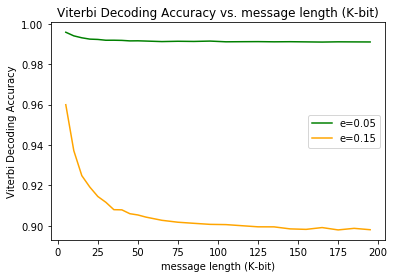
\includegraphics[width=0.8\linewidth]{img/viterbi.png}}
\end{center}
   \caption{Viterbi Accuracy over K-bit Message Length}
\end{figure}


\begin{figure}[t]
\begin{center}
\fbox{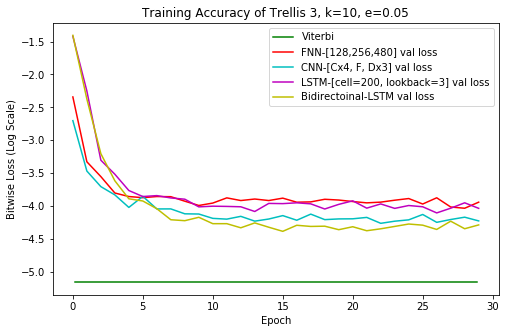
\includegraphics[width=0.8\linewidth]{img/k10-e05.png}}
\end{center}
   \caption{Short Message Length and Low Channel Corruption}
\end{figure}


\begin{figure}[t]
\begin{center}
\fbox{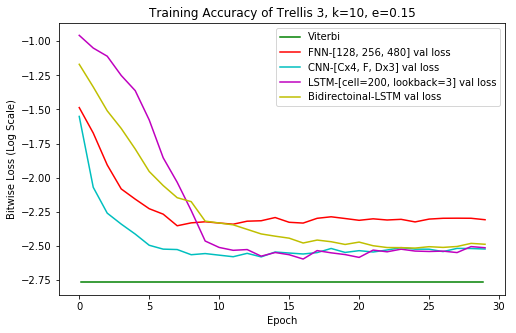
\includegraphics[width=0.8\linewidth]{img/k10-e15.png}}
\end{center}
   \caption{Short Message Length and High Channel Corruption}
\end{figure}


\begin{figure}[t]
\begin{center}
\fbox{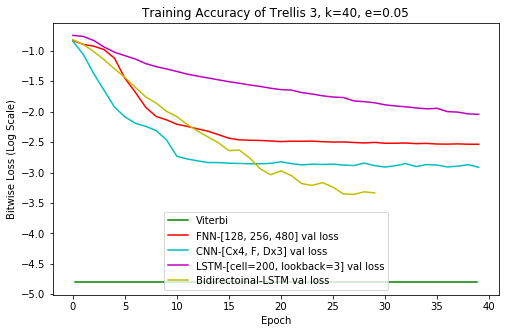
\includegraphics[width=0.8\linewidth]{img/k40-e05.png}}
\end{center}
   \caption{Long Message Length and Low Channel Corruption}
\end{figure}

%-------------------------------------------------------------------------

\section{Discussions}

In this section, I will compare and evaluate different architecture performance in terms of the bitwise accuracy compared to both the ground truth and the optimal Viterbi decoding algorithm accuracy. Other metrics such as the hamming distances to the ground truth, performance against K nearest neighbor and do-nothing approaches are also examined but not included in this report, as it's the work mainly done by another team member. 

\subsection{Results}

Specifically, Table 1 below shows the \textit{bitwise test accuracy} among various architectures trained over 30-40 epochs on three different scenarios with varying message length and channel corruption probability. Figure 1 shows the Viterbi Accuracy against the encoded message length $k$. Figure 2 shows the \textit{bitwise validation accuracy} of all five approaches (plotted in log scale) over the training epochs when the message length is short ($k=10$) and the channel corruption probability is low ($p=0.05$). Figure 3 shows that of short message length ($k=10$) but high channel corruption probability ($p=0.15$). Figure 4 shows that of a long message length ($k=40$) but low channel corruption probability ($p=0.05$). Note that the case of long message length and high channel corruption case is intentionally left out in this report, because empirically all four deep network architectures except the Viterbi algorithm seem to perform badly in this scenario, so I suspect more architectures design efforts are required for a actually interesting result.

\subsection{Architecture Performances}

In general, Viterbi algorithm performs the most optimal, as expected, among all methods, achieving generally around 99.1\% to 99.4\% bitwise accuracy in the low channel corruption probability case and around 93.7\% bitwise accuracy in the high channel corruption probability case. The length of the messages $k$ doesn't affect the Viterbi accuracy as much when the message is short but it indeed has a negative effect on the Viterbi performance slightly in the high channel corruption probability case.

FNNs don't perform as well as other more sophisticated neural network architectures. While it performs similarly well in the case of short message length and low channel corruption probability, achieving around 98.17\% bitwise validation accuracy, its performance diverges from other architectures as the decoding task becomes harder, either in terms of longer message length or more noisy inputs.

Interestingly and unintuitively, but not quite surprisingly, CNNs perform better than basic RNN-LSTM in all three cases tested with \textit{both faster convergence rate and better bitwise accuracy}. One possible explanation is that even more architecture search and design efforts are needed for the basic RNN-LSTM case. Or maybe the nature of the convolution operation inside the convolutional encoding incorporates more information about the original message than the time-sequential nature of the encoding, so CNN is better suited for the task and can pick up more hidden patterns than basic RNN-LSTM.

However, as we can see from the plots and the table, although CNN outperforms basic RNN-LSTM consistently, Bidirectional LSTM competes with CNNs with comparable performance and convergence rate. Specifically, in a short message length case regardless of the channel corruption probability, Bidirectional LSTM performs comparably well as CNNs. Note that their relevant accuracy has a slight variance depending on the data tested (as seen from either tested on the validation and test set) and their performance are actually very close. I would conclude both architectures perform in equal grounds as the small difference in performance probably results from the data set variance. 

Bidirectional LSTM, nevertheless, performs significantly better in terms of bitwise accuracy than CNN in the long message length and high channel corruption case, as shown in Figure 4, but CNN converges faster than Bidirectional LSTM. One possible explanation for why Bidirectional LSTM performs better than LSTM is that Bidirectional LSTM brings information from the future into considerations while LSTM doesn't. Since convolutional encoding has the time sequential nature and certain states are not possible as we advance and encode according to the Trellis diagram, examining the state of the encoding from both the past and the future in Bidirectional LSTM will help make more informative decision on the current prediction and determine which noisy bits are probably corrupted, thus leading to higher bitwise accuracy even in the high channel corruption probably case, explaining Bidirectional LSTM's edge over the CNN.


\subsection{Proposed ResNet-based Architecture}

One experimental architecture that I intended to experiment but haven't got the chance yet is a two-stage pipeline consisting of a denoising stage and a decoding stage.

\subsection{Denoising}

Since channel corruption generally flips random bits in the sent-over, convolutionally-encoded sequence, it makes sense intuitively to train a ResNet-based architecture to denoise the noisy corrupted convolutional sequence as the first stage in the pipeline. The rationale is that learning a residual to predict which bits are corrupted should be easier to train than learning to completely generate a new sequence from scratch.

One baseline that can be used as a comparison to the performance of the denoising stage is k nearest neighbor, where k nearest neighbor will choose which original uncorrupted sequence is most likely given a sequence of noisy sequence. As we have more training data, k nearest neighbor should converge to a baseline performance accuracy. However, k nearest neighbor doesn't perform well in a high dimensional case due to the curse of dimensionality, so we don't expect k nearest neighbor to perform well as the denoising baseline when message length is long. However, one alternative that one may use is to have a fixed-length sliding window on the noisy input sequence and concatenates the k nearest neighbor output together.

\subsection{Decoding}

Once we have a deep-network denoised convolutional encoding, we use a second neural network to decode it as if the input is uncorrupted. Essentially, we will try to find a neural network architecture to approximate the performance of the Viterbi decoding algorithm in decoding uncorrupted convolutional code. It should be slightly easier as the second-stage deep neural networks now don't need to denoise and decode both at the same time, but focus on only making the decoding task well.

\subsection{End-to-End}

Having developed and trained a high-performing two-stage pipeline as described above, we can then go ahead and figure out if there is a way to combine them into an end-to-end architecture. We probably can take insights from FCN, Faster R-CNN, YOLO 2, etc. to, for example, output locations of bits that are probably corrupted and propose possible decoding at the same time.


%-------------------------------------------------------------------------
\section{Semester Reflection}

\subsection{Mistakes}

For error correction, I started out experimenting with basic Feed Forward Networks. For the first few weeks, I made mistakes of either using too few training data (around 1000 data points only), or not linearly scaling the hidden layers as message length $K$ increases. These two mistakes lead to significant underfitting of the models. However, I quickly fixed the mistake and retrained my deep neural network models.

Also, the plot of Bidirectional LSTM is cut off at epoch 30 because of my computer died at that point, and I didn't get to retrain it as it takes quite some time to train these models in the long message length and high channel corruption case, and we cannot \textit{just} retrain the Bidirectional-LSTM because the data will have been shuffled different when I restart my notebook. To keep the model performance meaningful, I need to use the same train-validation-test split to test the model, so it will require me to retrain all four models. However, even so, we can clearly see already how Bidirectional-LSTM is beating other neural network architectures even at epoch 30. In future, I would keep more frequent checkpoints for models and save the pre-processed data sets so we can easily retrain and repeat experiments


\subsection{What I Have Learned}

In this semester (Spring 2018) of research, I learned many possible ways to compare the performance of neural network architectures. I learned that obtaining seemingly high accuracy doesn't necessary mean the neural network is doing well, because traditional machine learning methods such as k nearest neighbor may already perform better. I also learned other not commonly used loss metrics such as Hamming distance to target output, or comparisons to do-nothing approach. I also learned a lot about the realm of wireless communication and the radio domain, which I've never explored before. I also learned how to examine and gain insights from poor neural network results and explore new directions based on the experiments. Listening to the feedback that Professor Sahai give to all three different teams really give insights as what it is like to be a disciplined machine learning researcher, and of course I can improve a lot by learning from other people's mistakes and approaches.

\end{document}
